%%%%%%%%%%%%%%%%%%%%%%%%%%%%%%%%%%%%%%%%%%%%%%%%%%%%%%%%%%%%%%%%%%%%%%%%%%%%%%%%
% Template for USENIX papers.
%
% History:
%
% - TEMPLATE for Usenix papers, specifically to meet requirements of
%   USENIX '05. originally a template for producing IEEE-format
%   articles using LaTeX. written by Matthew Ward, CS Department,
%   Worcester Polytechnic Institute. adapted by David Beazley for his
%   excellent SWIG paper in Proceedings, Tcl 96. turned into a
%   smartass generic template by De Clarke, with thanks to both the
%   above pioneers. Use at your own risk. Complaints to /dev/null.
%   Make it two column with no page numbering, default is 10 point.
%
% - Munged by Fred Douglis <douglis@research.att.com> 10/97 to
%   separate the .sty file from the LaTeX source template, so that
%   people can more easily include the .sty file into an existing
%   document. Also changed to more closely follow the style guidelines
%   as represented by the Word sample file.
%
% - Note that since 2010, USENIX does not require endnotes. If you
%   want foot of page notes, don't include the endnotes package in the
%   usepackage command, below.
% - This version uses the latex2e styles, not the very ancient 2.09
%   stuff.
%
% - Updated July 2018: Text block size changed from 6.5" to 7"
%
% - Updated Dec 2018 for ATC'19:
%
%   * Revised text to pass HotCRP's auto-formatting check, with
%     hotcrp.settings.submission_form.body_font_size=10pt, and
%     hotcrp.settings.submission_form.line_height=12pt
%
%   * Switched from \endnote-s to \footnote-s to match Usenix's policy.
%
%   * \section* => \begin{abstract} ... \end{abstract}
%
%   * Make template self-contained in terms of bibtex entires, to allow
%     this file to be compiled. (And changing refs style to 'plain'.)
%
%   * Make template self-contained in terms of figures, to
%     allow this file to be compiled. 
%
%   * Added packages for hyperref, embedding fonts, and improving
%     appearance.
%   
%   * Removed outdated text.
%
%%%%%%%%%%%%%%%%%%%%%%%%%%%%%%%%%%%%%%%%%%%%%%%%%%%%%%%%%%%%%%%%%%%%%%%%%%%%%%%%

\documentclass[letterpaper,twocolumn,10pt]{article}
\usepackage{usenix2019_v3}

% to be able to draw some self-contained figs
\usepackage{tikz}
\usepackage{amsmath}
\usepackage{xcolor}
\usepackage{graphicx}
\usepackage{subcaption}
\usepackage{float}
\usepackage{listings, multicol}

% inlined bib file
\usepackage{filecontents}

\lstdefinelanguage{P4}{
  keywords={in, out, struct, inout, function, return, switch, enum, if, else, case, break, extern, void, bit, error, int, verify, bool, key, table, action, actions, parser, control, state, transition, select, apply},
  keywordstyle=\color{myk}\bfseries,
  keywords=[2]{boolean, string, number, objectid},
  keywordstyle=[2]\color{green}\bfseries,
  identifierstyle=\color{darkgray}\bfseries,
  sensitive=false,
  comment=[l]{//},
  morecomment=[s]{/*}{*/},
  commentstyle=\color{commentcolor}\ttfamily,
  stringstyle=\color{red}\ttfamily,
  morestring=[b]',
  morestring=[b]"
}

\lstset{
   language=P4,
%    numbers=left,
%    backgroundcolor=\color{mygray},
   extendedchars=true,
   basicstyle=\small\ttfamily\color{darkgray}\bfseries,
   showstringspaces=false,
   showspaces=false,
   tabsize=2,
   frame=single,
   breaklines=true,
   showtabs=false
}
\definecolor{mygray}{gray}{1.0}
\definecolor{commentcolor}{RGB}{0,100,0}
\definecolor{myk}{rgb}{0.0,0,0.65}

\newcommand{\hs}[1]{{\color{blue}{HS:#1}}}

% %-------------------------------------------------------------------------------
% \begin{filecontents}{\jobname.bib}
% %-------------------------------------------------------------------------------
% @Book{arpachiDusseau18:osbook,
%   author =       {Arpaci-Dusseau, Remzi H. and Arpaci-Dusseau Andrea C.},
%   title =        {Operating Systems: Three Easy Pieces},
%   publisher =    {Arpaci-Dusseau Books, LLC},
%   year =         2015,
%   edition =      {1.00},
%   note =         {\url{http://pages.cs.wisc.edu/~remzi/OSTEP/}}
% }
% @InProceedings{waldspurger02,
%   author =       {Waldspurger, Carl A.},
%   title =        {Memory resource management in {VMware ESX} server},
%   booktitle =    {USENIX Symposium on Operating System Design and
%                   Implementation (OSDI)},
%   year =         2002,
%   pages =        {181--194},
%   note =         {\url{https://www.usenix.org/legacy/event/osdi02/tech/waldspurger/waldspurger.pdf}}}
% \end{filecontents}
% 
%-------------------------------------------------------------------------------
\begin{document}
%-------------------------------------------------------------------------------

%don't want date printed
\date{}

% make title bold and 14 pt font (Latex default is non-bold, 16 pt)
\title{\Large \bf Formatting Submissions for a USENIX Conference:\\
  An (Incomplete) Example}

%for single author (just remove % characters)
\author{
{\rm Your N.\ Here}\\
Your Institution
\and
{\rm Second Name}\\
Second Institution
% copy the following lines to add more authors
% \and
% {\rm Name}\\
%Name Institution
} % end author

\maketitle

%-------------------------------------------------------------------------------
\begin{abstract}
%-------------------------------------------------------------------------------
Your abstract text goes here. Just a few facts. Whet our appetites.
Not more than 200 words, if possible, and preferably closer to 150.
\end{abstract}


\section{Introduction}

% hardware and software together, cool
Over the last decade, the synergistic development of packet-processing
hardware and software has fundamentally changed how networks are built
and operated. Hardware platforms such as
RMT~\cite{Bosshart:2013:FMF:2486001.2486011} provide tremendous
flexibility for customizing the forwarding plane without having to
fabricate new chips, while languages such as
P4~\cite{Bosshart:2014:PPP:2656877.2656890, p4lang} enable programmers
to describe rich packet-processing functions in terms of high-level
abstractions such as parsers and match-action tables.

In order to support different kinds of targets (e.g., software
switches, ASICs, FPGAs, etc.), P4 allows programmable and
fixed-function blocks to be arranged into different layouts as
specified by an architecture declaration. For example, the Protocol
Independent Switch Architecture
(PISA)~\cite{Bosshart:2013:FMF:2486001.2486011} models a switch with a
programmable parser, programmable ingress pipeline, fixed-function
scheduler and queues, programmable egress pipeline, and programmable
deparser. PISA programs supply P4 code for each programmable block.
But while this design allows the language to flexibly accommodate a
wide range of targets, it also creates a tight coupling between
programs and architectures, which makes it difficult to write programs
in a compositional manner or reuse common code fragments in different
programs.

For example, \texttt{switch.p4}~\cite{switch.p4} handles several dozen
different protocols and functions (e.g., L2 switching, L3 routing,
tunneling, etc.,). But the code is written against a global collection
of q metadata and parsed headers. To use the code in
\texttt{switch.p4} to implement an Ethernet switch, it would be
necessary to detangle the L2-specific functionality from the
extraneous code in the rest of the program. Without a detailed
understanding of the overall structure of the top-level program, it is
difficult or impossible to reuse code fragments at finer granularity.

% \section{Use Case}
Consider a simple scenario, as shown in Figure~\ref{fig:l3.p4.l2.p4}.
The first program, \texttt{l3.p4}, parses the IPv4 header, uses
longest-prefix matching to determine the next hop, decrements the
\texttt{ttl} field and, finally, deparses the packet. The second
program, \texttt{l2.p4}, parses the Ethernet header, and modifies the
ethernet addresses using the next hop, which is supplied as an
argument, and finally deparses the packet. Note that neither
\texttt{l3.p4} nor \texttt{l2.p4} is a complete packet-processing
program: the former does not generate a functionally correct packets,
while the latter is parameterized on the next hop and so does not
specify forwarding behavior. However, we could combine \texttt{l2.p4}
with any other routing scheme (e.g., IPv6, MPLS, etc.) to obtain a
valid program. 

\begin{figure*}[!ht]
\noindent \begin{minipage}[t]{.48\textwidth}
\begin{lstlisting}[frame=none]
// l3.p4
struct meta_t { bit<16> type; }
parser P(packet_in pin, out hdr_t hdrs, inout meta_t m) {
  state start {
    transition select(m.type){
       0x0800: parse_ipv4;
    }
  }
  state parse_ipv4 {
      pin.extract(hdrs.ipv4);
      transition accept;
  }
}
control Pipe(inout hdr_t hdrs, out bit<16> nexthop_id, inout sm_t sm) {
  action process(bit<16> nh) {
    hdrs.ipv4.ttl = hdrs.ipv4 - 1;
    nexthop_id = nh;// setting out param
  }
  table ipv4_lpm_tbl {
    key = { hdrs.ipv4.dstAddr : lpm } 
    actions = { process; }
  }
  apply { ipv4_lpm_tbl.apply(); }
}
control D(packet_out po, in hdr_t hdrs) {
  apply { po.emit(hdrs.ipv4); }
}
\end{lstlisting}
\end{minipage}\vline
\hfill\begin{minipage}[t]{.48\textwidth}
\begin{lstlisting}[frame=none]
// l2.p4
parser P(packet_in pin, out hdr_t hdrs) {
  state start {
    pin.extract(hdrs.eth);
  }
}
control Pipe(inout hdr_t hdrs, inout sm_t sm, 
             in bit<16> nexthop_id) {
  action drop () {}           
  action forward(bit<48> dest_mac, 
                 bit<48> src_mac, bit<8> port) {
    hdrs.eth.dstAddr = dest_mac;
    hdrs.eth.srcAddr = src_mac;
    sm.out_port = port;    
  }
  table forward_tbl {
    key = { nexthop_id : exact; } 
    actions = { process; drop; }
  }
  apply {
    forward_tbl.apply(); 
    if (sm.deq_qdepth > 100) // rate limiting
      drop();
  }
}
control D(packet_out po, in hdr_t hdrs) {
  apply { po.emit(hdrs.eth); }
}
\end{lstlisting}
\end{minipage}
% \vspace*{-10pt}
\caption{Example: \texttt{l3.p4} and \texttt{l2.p4}.}
\label{fig:l3.p4.l2.p4}
\end{figure*}


%% The current ecosystem of programmable data plane enforces programmers
%% to write code amenable to the target device's data plane architecture
%% and pipeline. Programmers write code for programmable blocks taking
%% into account their location in pipeline rather than compilers
%% automatically allocating code to the appropriate blocks. We believe
%% that devices should only expose abstraction for processing blocks and
%% the onus of code allocation to the blocks in pipeline should be on
%% compilers for the devices.

There is some prior work on modular composition of P4 programs.
Systems such as HyPer4 \cite{Hancock:2016:HUP:2999572.2999607},
HyperV~\cite{8038396}, and
P4Visor~\cite{Zheng:2018:PLV:3281411.3281436} provide constructs for
merging independent programs onto a single device. However, these
systems only handle programs that describe end-to-end
packet-processing functions. Hence, they lack mechanisms for enabling
selective reuse of library code, specifying interfaces between
modules, and facilitating inter-module communication. To write truly
modular P4 programs, a fundamentally different approach is needed.

To this end, this paper presents the design and (prototype)
implementation of $\mu$P4, a new architecture that provides
fine-grained abstractions for constructing data plane programs.
$\mu$P4 consists of two components, Micro Switch Architecture
($\mu$SA), which distills packet processing to its essence, and
abstracts away from device-specific structure, and a compiler,
$\mu$P4C, that maps one or more $\mu$SA programs to a standard PISA
pipeline. 

This paper makes the following contributions.
\begin{itemize}
\item We motivate the need for modular data plane programming using a
  series of realistic examples.
\item We introduce $\mu$ SA, a new P4 architecture designed to enable
  fine-grained composition of program snippets.
\item We develop techniques for compiling $\mu$SA programs to the
  standard PISA model, including merging programs composed together in
  parallel or in sequence onto a single PISA pipeline.
\end{itemize}

Although much work remains, we believe that $\mu$ SA represents a
promising first step toward enabling modular data plane programs.

\section{Micro-Switch Architecture}
\label{section:micros-awitch-architecture}
The design goals behind $\mu$SA are $(1)$ provide logical abstraction for data plane pipelines without compromising expressiveness and packet-processing features, $(2)$ declare generic interfaces to allow easy code reuse and enable modularity.
First, we describe logical pipelines of $\mu$P4. Then, we introduce $\mu$SA's externs and generic interfaces along with example usages.

% This design choice reduces heterogeneity in abstract model of data plane programs.
% For each pipeline type, it exposes an interface type comprising a set of programmable blocks.
% Programmers can define a P4 \emph{package} type by implementing all the programmable blocks of a interface type.
% In the same source file, programmers can provide multiple implementations of the same interface type to define multiple package types.
% $\mu$SA defines various architecture specific structures and externs that allow programmers to express sequential and parallel composition of fine-grained packet processing functions.

% It defines standard intrinsic metadata as \emph{msa\_sm\_t} as a struct type.
% The fields of this struct provide basic information populated by the target e.g., \emph{packet\_length}.

% Some fields are not mutable, however $\mu$SA allows to declare instances of the struct and perform assignment operation between two instances to create copies.
% Sections \ref{subsection:pipelines} and \ref{subsection:logical-externs} describe pipelines and logical externs, respectively.

\begin{figure}
    \centering
    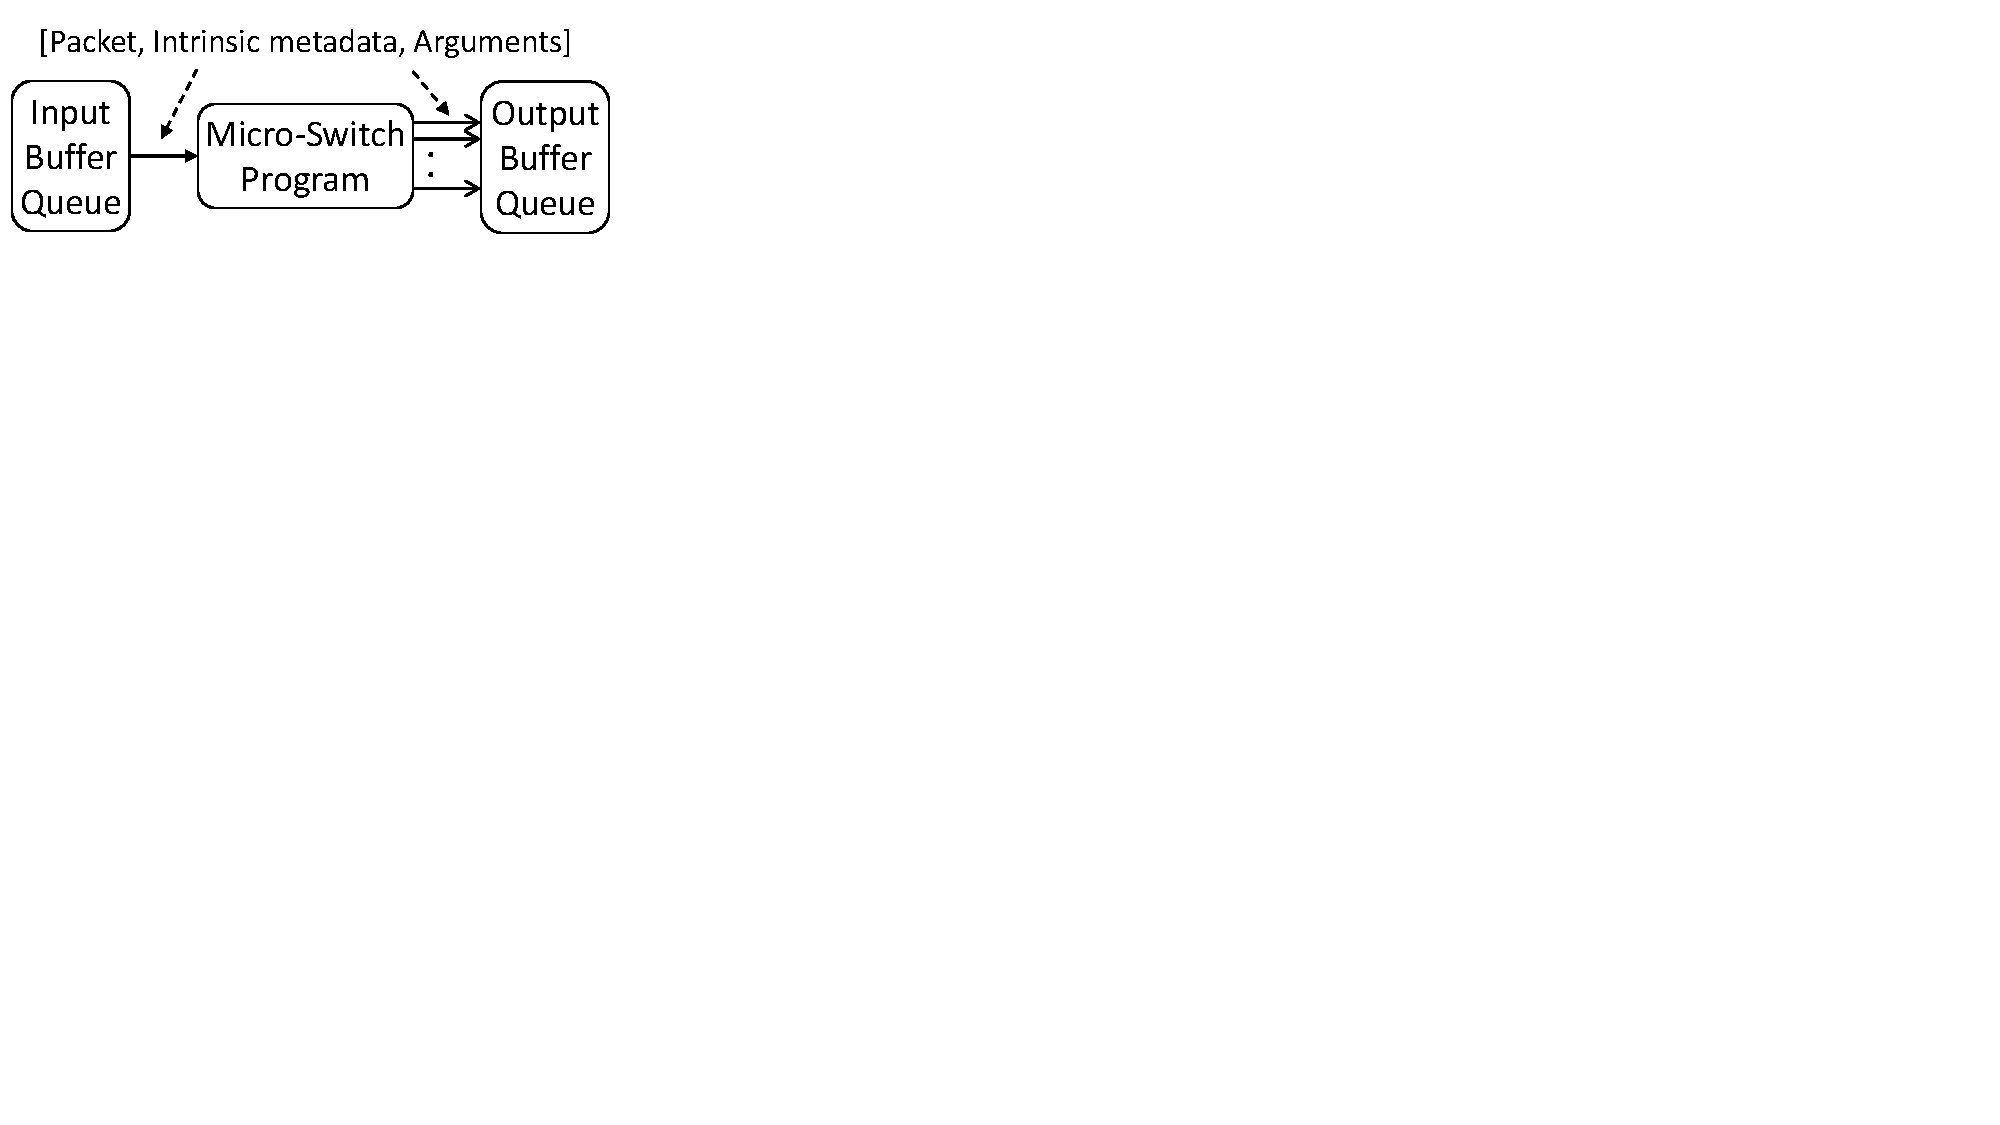
\includegraphics[trim=0 420 667 0, clip, scale=0.5]{microp4-program-model}
    \caption{$\mu$P4 Packet Processing model}
    \label{fig:mp4-packet-processing-model}
\end{figure}

\subsection{Pipelines}
\label{subsection:pipelines}
$\mu$SA has two types logical pipeline, Micro and Orchestration, shown in Figure \ref{fig:msa-pipelines}
$\mu$SA provides a set of logical externs which can be instantiated and used within control blocks of the $\mu$SA pipelines.
Micro pipeline comprises of Parser, Micro-Pipe control and Deparser programmable blocks.
$\mu$SA does not allow conditional statements in deparser blocks.
% Every incoming packet is parsed and validated by the parser, if parser terminates in \texttt{accept} state, then execution-control is transferred to micro-pipe control block.
% Depending on use of logical externs in implementation, packet may not complete the processing of the control block.
% If the execution-control reaches till the end of the control block, packet is processed by the deparser block.
\begin{figure}[H]
    \centering
    \begin{subfigure}{0.59\linewidth}
        \centering
        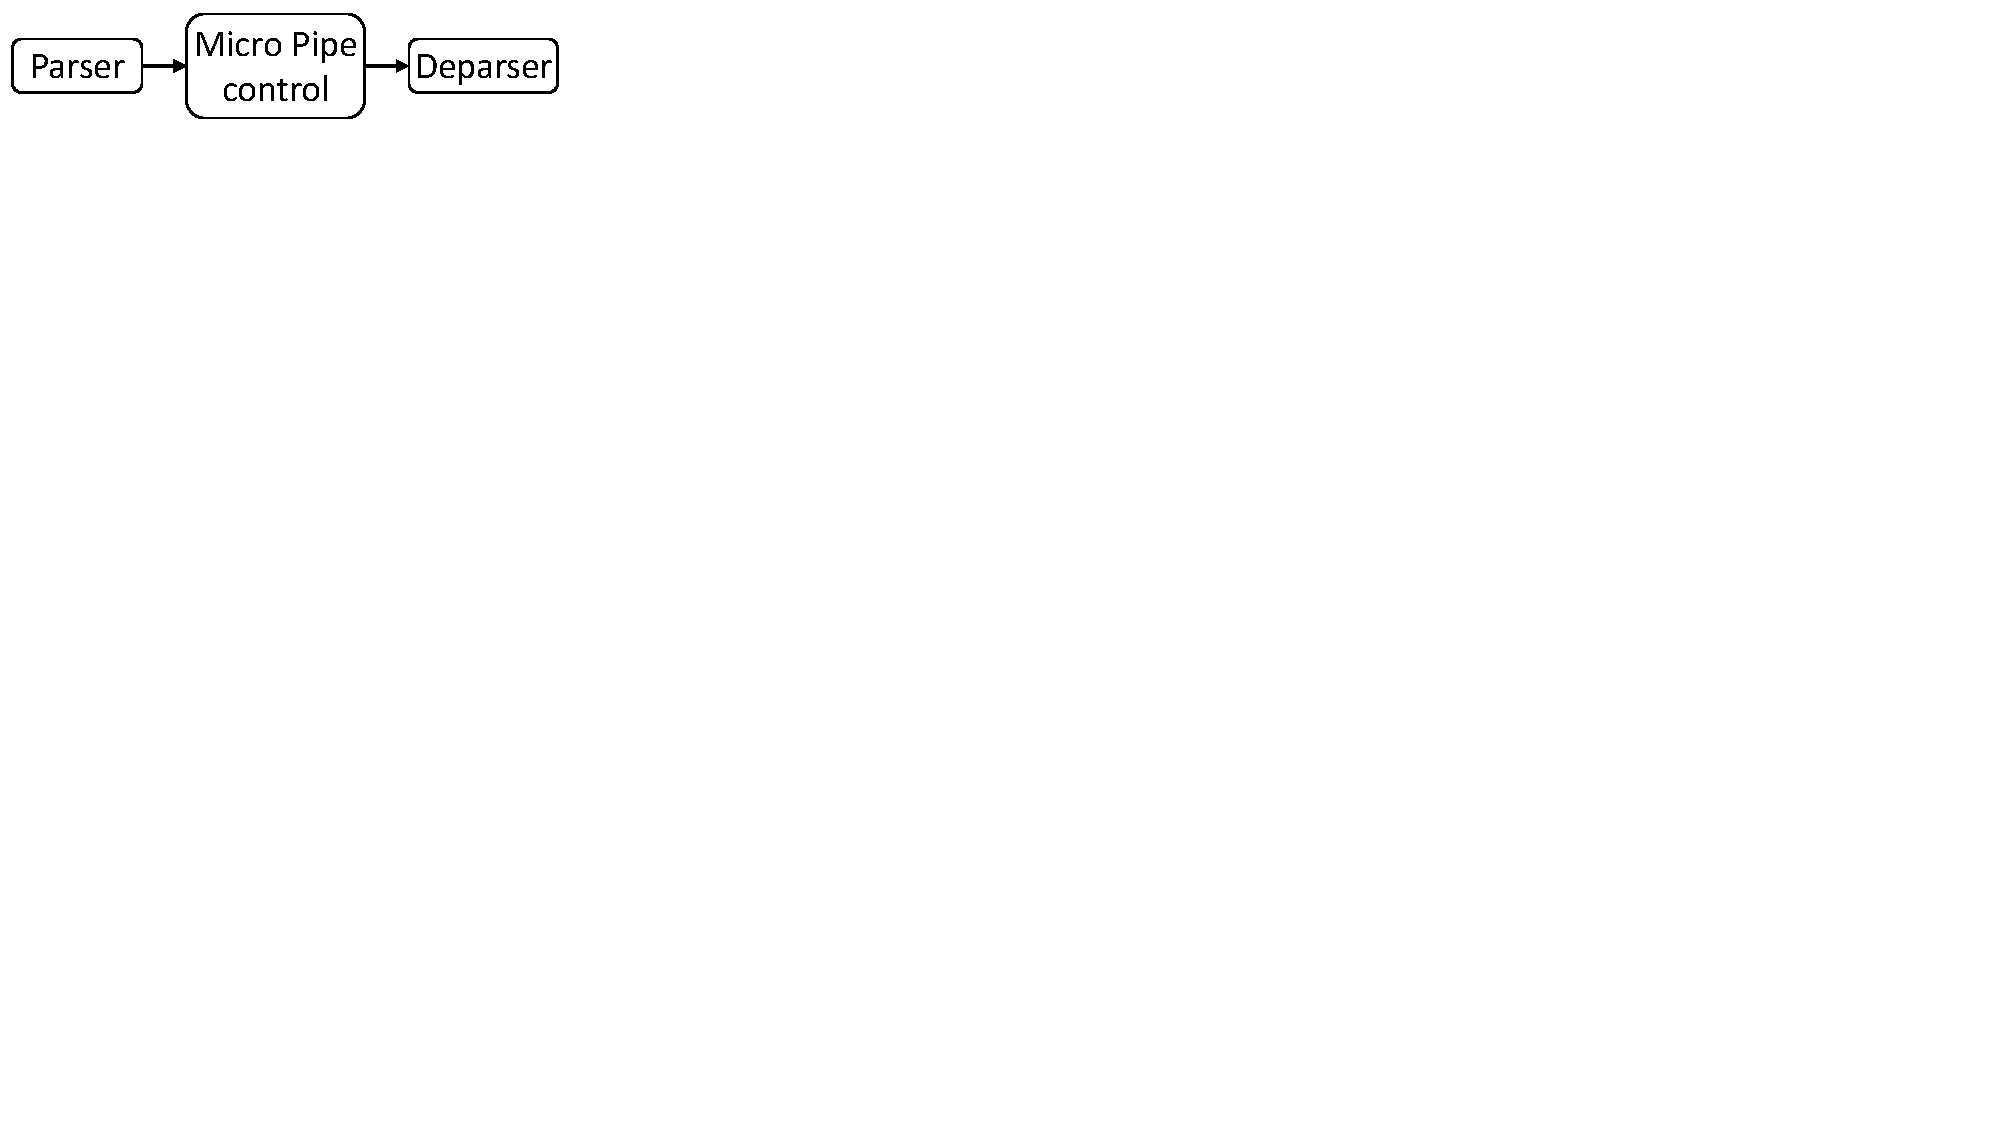
\includegraphics[trim=0 482 692 0, clip,scale=0.45]{msa-pipeline}
        \caption{Micro}
%         \label{subfig:micro}
    \end{subfigure}\vline
    \begin{subfigure}{0.41\linewidth}
        \centering
        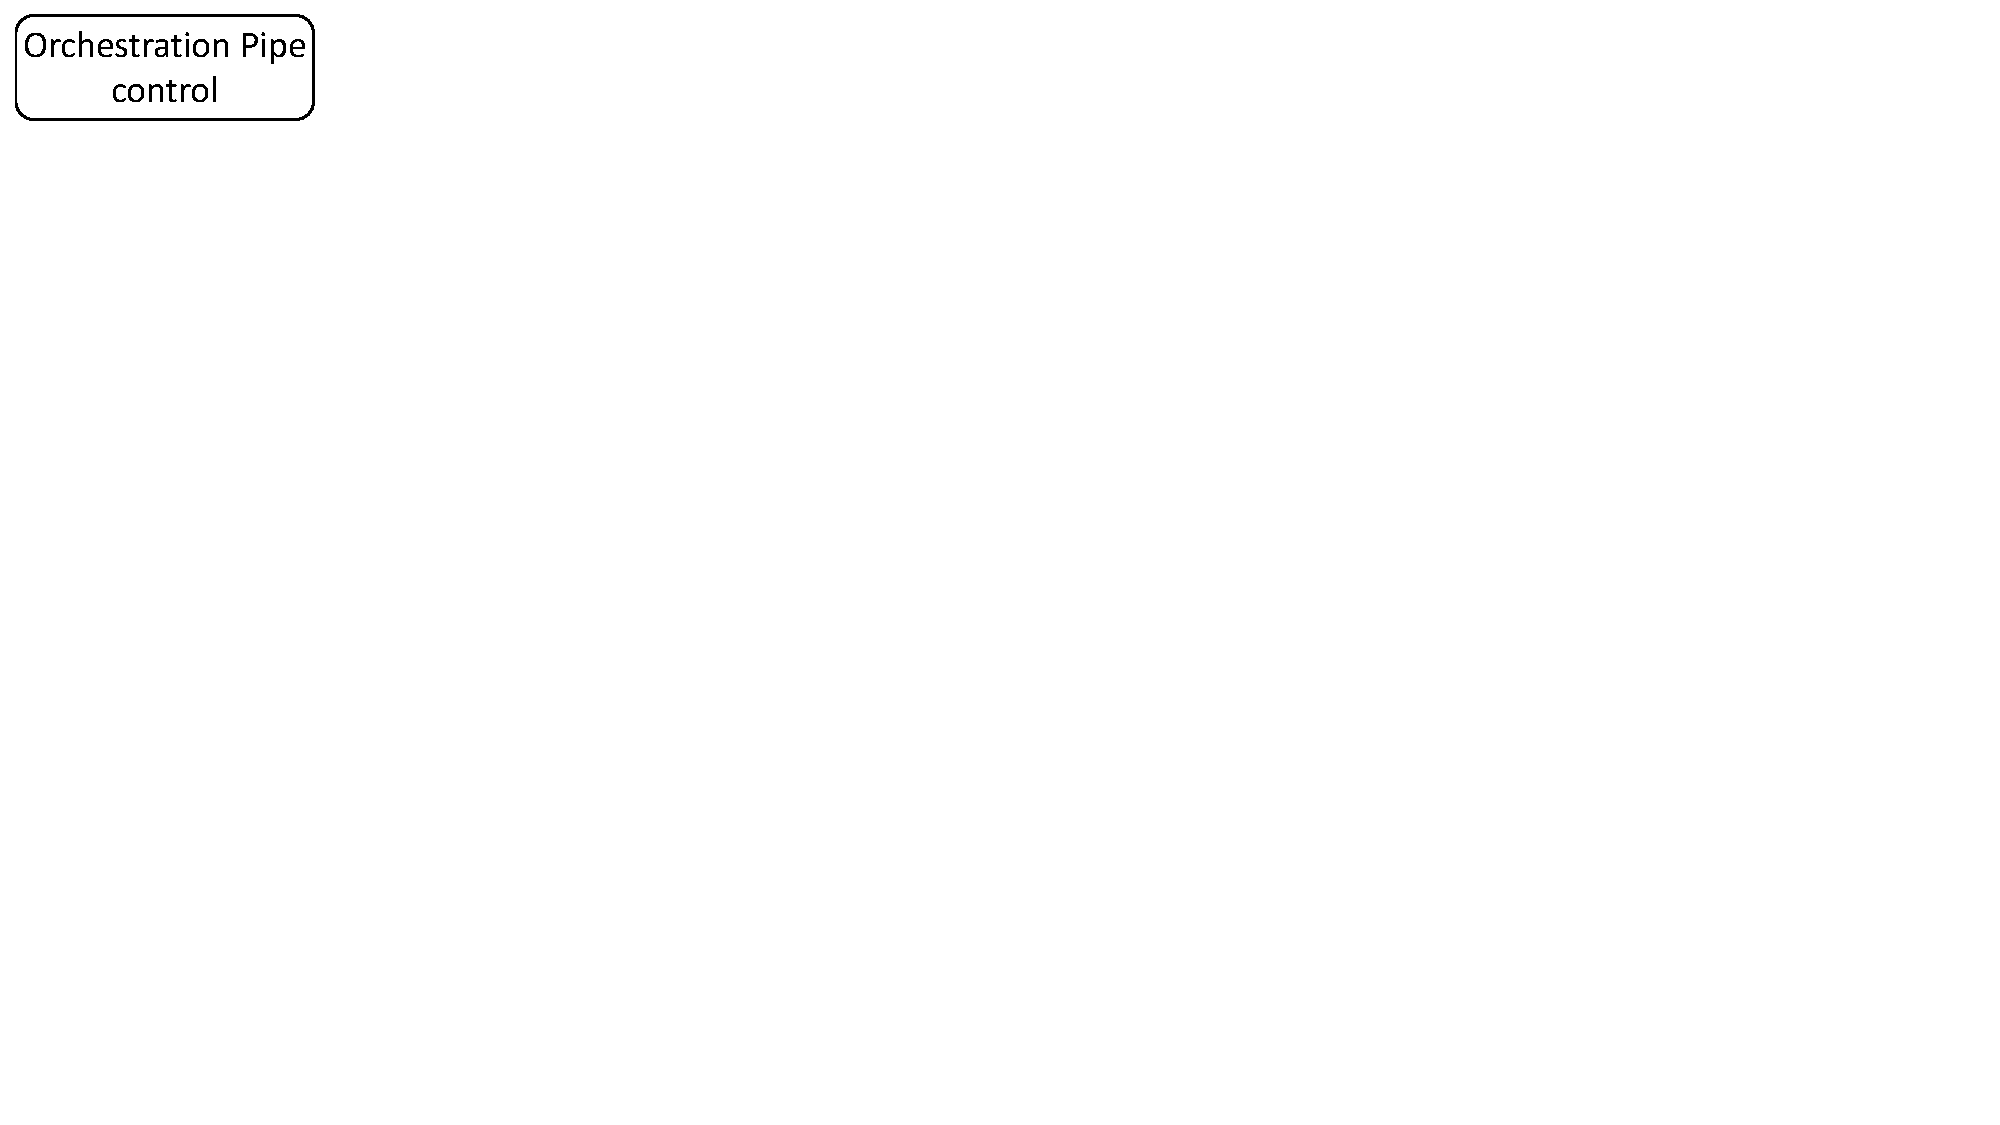
\includegraphics[trim=0 480 805 0,clip,scale=0.45]{micro-orchestration-pipeline}
        \caption{Orchestration}
%         \label{subfig:orchestration}
    \end{subfigure}
\caption{$\mu$SA Pipelines}
\label{fig:msa-pipelines}
\end{figure}
% \vspace{-3pt}
Orchestration pipeline only has a control block, orchestration pipe.
Programmers can implement imperative control flow using intrinsic metadata of $\mu$SA and runtime parameters to the package types.

Figure \ref{fig:interfaces} shows signature of type-parameterized interfaces declared in $\mu$SA.
Unicast (U) and Multicast (M) interface can be implemented using Micro pipeline.
General (G) interface allows to implement Orchestration pipeline.
In Figure \ref{fig:interfaces}, \texttt{pkt\_in} and \texttt{pkt\_out} represent packet, \texttt{sm\_t} and \texttt{es\_t} represent intrinsic metadata.
\texttt{in\_buf} and \texttt{out\_buf} externs represent input and output buffer of $\mu$P4 packet-processing model (Figure \ref{fig:mp4-packet-processing-model})
% \vspace{-7pt}
\begin{figure}[H]
\begin{lstlisting}[frame=none]
// Interfaces with apply method
Unicast<I, O, IO>(pkt, inout sm_t, es_t, 
    in I, out O, inout IO);
Orchestration<I, O>(in_buf<I>, out_buf<O>);
// Interface with fork method
Multicast<I, O>(pkt, in sm_t, es_t, in I, out_buf<O>);
\end{lstlisting}
\caption{Runtime Interfaces}
\label{fig:interfaces}
\end{figure}

\begin{figure}[ht]
\begin{lstlisting}[frame=none]
extern pkt {
  // byte array representation
}
extern emitter {
  void emit (pkt, in hdr);
  dettach(pkt);
}
extern extractor {
  void extractor(pkt, out hdr);
  /// T may be an arbitrary fixed-size type.
  T lookahead<T>();
}
\end{lstlisting}
\caption{Packet Representation}
\label{fig:pkt-externs}
\end{figure}
\begin{figure}[ht]
\begin{lstlisting}[frame=none]
extern in_buf<I> {
  dequeue(pkt, out sm_t, es_t, out I);
}
extern out_buf<O> {
  enqueue(pkt, in sm_t, es_t, in O);
}
extern mc_in_buf<H, I> {
  dequeue(pkt, out H, out sm_t, es_t es, out I);
}
extern mc_out_buf<H, O> {
  enqueue(pkt, in H, in sm_t, es_t es, in O);
}
\end{lstlisting}
\caption{Buffer Representation}
\label{fig:pkt-buf}
\end{figure}
\begin{figure}[ht]
\begin{lstlisting}[frame=none]
// This can only be used in control block of multicast interface
extern mc_engine {
  mc_engine();
  void set_mc_group(GroupId_t gid);
  apply(es_t, out PacketInstanceId_t);
  
  set_buf(out_buf<O>);
  apply(pkt, out sm_t, es_t, out O);  
}
\end{lstlisting}
\caption{Multicast Extern}
\label{fig:msa-multicast-extern}
\end{figure}
\begin{figure}[H]
\begin{lstlisting}[frame=none]
// Unicast
parser p<H, M, I, O, IO>(extractor, pkt, H, M, I, O, IO, sm_t, es_t);
control c<H, M, I, O, IO>(pkt, H, M, I, O, IO, sm_t, es_t);
control d<H, M>(emitter, pkt, H);

Unicast<H, M, I, O, IO>
  (pkt, inout sm_t, es_t, in I, out O, inout IO) // runtime params
  (p<H, M, I, O, IO>, c<H, M, I, O, IO>, d<H, M>); // compile-time params


// Multicast
parser p<H, M, I>(extractor, pkt, H, M, I, sm_t, es_t);
control c<H, M, I, O)>(pkt, H, M, I, sm_t, es_t, mc_out_buf<H,O>);
control d<H, O> (emitter, out_buf<O>, mc_in_buf<H,O>);

// Orchestration
control c<I, O)>(pkt, sm_t, es_t, in I, out_buf<O>);
    
\end{lstlisting}
\caption{Programmable Blocks for Interfaces}
\label{fig:programmable-blocks-for-interfaces}
\end{figure}

\subsubsection{Multicast Execution}
\label{subsubsection:multicast-execution}
Multicast execution differs from parallel execution in two fundamental aspects.
$(1)$ Multicast execution allows to program packet replication at runtime.
$(2)$ Each copy of the replicated packet executes the same code.
% $\mu$SA defines a logical multicast engine, \texttt{mc\_engine\_t}, as an extern.
Figure \ref{fig:multicast-execution} shows an example of expressing multicast replication using logical externs defined in $\mu$SA.



\subsubsection{Multicast Extern}
$\mu$SA's multicast extern (Figure \ref{fig:msa-multicast-extern}) can be instantiated in the control blocks of its pipelines.
The \emph{set\_multicast\_group} can be used to assign replication group to the packet. 
The \emph{apply} function is allowed to use only in \emph{apply} body control blocks. 
It is analogous to \emph{fork} system call in C except that processing of original packet terminates at the apply call.
It returns instance id of the replica and populates the es\_t instance with the port id set by the control plane.
$\mu$P4C translates this extern to multicast mechanism defined in architectures of real targets.
% We assume these architectures would have sufficient fields to program their replication engine, so that a combination of the fields can be used as packet instance id.


% \begin{figure}[H]
% \begin{lstlisting}
% struct out_t { bit<16> data;}
% control mc(pkt_in pi, sm_t sm, es_t es, 
%         hs_t h, ia_t ia, mc_buf<hs_t, out_t> hb) {
%   mc_engine mce;  pkt_inst_id_t id; 
%   out_t  oa;
%   table t{
%     key = {} actions = { mce.set_mc_group; drop; }
%   }
%   table mac{
%     key = { es.get_port(); } 
%     actions = { mac_update; }
%   }
%   apply {
%     id = mce.apply(es); // equivalent to fork in C
%     mac.apply();
%     hb.enqueue(h, sm, es, oa);
%   }
% }
% control dep(pkt_out<o_a> ob, 
%             mc_buf<hs_t, out_arg_t> hb) {
%   hs_t hdrs; out_arg_t oa; pkt_out po;
%   hb.dequeue(hdrs, sm, es, oa);
%   // deparser code 
%   ob.enqueue(po, sm, es, oa);
% }
% \end{lstlisting}
% \caption{Multicast Execution}
% \label{fig:multicast-execution}
% \end{figure}

\subsection{Logical Externs and Examples}

\subsubsection{Egress Specifications}
Many packet-processing devices allow to measure every packet's queuing latency through the device.
These timestamps required to compute queuing latency can be measured only after the packet's egress port is finalized.
The timestamps can be accessed only after the egress port is finalized.
$\mu$SA captures such constraints as using stateful extern objects capturing data-dependency.
% To support such special features, the architectures of real target devices expose intrinsic metadata  that depends on operations on other intrinsic metadata.
\begin{figure}[H]
\begin{minipage}[c]{\linewidth}
\begin{lstlisting}[frame=none]
enum meta_t {
  INGRESS_TIMESTAMP,
  EGRESS_TIMESTAMP
}
\end{lstlisting}
\end{minipage}
\begin{minipage}[c]{\linewidth}
\begin{lstlisting}[frame=none]
extern es_t {
  void set_egress_port(in bit<8>);
  bit<8> get_egress_port();
  bit<32> get_value(in meta_t ft);
  void copy_from(es_t es);
}
\end{lstlisting}
\end{minipage}
\caption{Extern to Capture Data-Dependency(Egress\_Spec)}
\label{fig:msa-egress-spec-extern}
\end{figure}
$\mu$SA declares \texttt{es\_t} as an extern object (Figure \ref{fig:msa-egress-spec-extern}).
It declares methods to manipulate and access interdependent device-specific information.
$\mu$P4C uses their occurrences to transform the code to multi-control pipelines of real target architectures.

% $\mu$P4C allows repeated usage of the extern's functions in the single control block of $\mu$SA pipelines.
% If \emph{get\_value} occurs before \emph{set\_egress\_port} on any possible execution-control path, $\mu$P4C raises a compile-time error.


\subsubsection{Packet Externs}

\begin{figure*}[!ht]
\noindent \begin{minipage}[t]{.50\textwidth}
\begin{lstlisting}[frame=none]
// l3 runtime interface
l3(pkt, inout sm_t, es_t, out bit<16>, inout bit<16>);
// l3.p4
parser P(extractor ex, pkt p, out l3_hdr_t hdr, inout bit<16> type) { //inout arg
  state start {
    transition select(type){
      0x0800: parse_ipv4;
    }
  }
  state parse_ipv4 {
    ex.extract(p, hdr.ipv4);
    transition accept;
  }
}
control Pipe(pkt p, inout l3_hdr_t hdr, out bit<16> nexthop, inout sm_t sm, es_t es) { // nexthop out arg
  action process(bit<16> nh) {
    hdrs.ipv4.ttl = hdr.ipv4 - 1;
    nexthop = nh;// setting out param
  }
  table ipv4_lpm_tbl {
    key = { hdr.ipv4.dstAddr : lpm } 
    actions = { process; }
  }
  apply { ipv4_lpm_tbl.apply(); }
}
control D(emitter em, pkt p, in l3_hdr_t h) {
  apply { em.emit(p, h.ipv4); }
}
\end{lstlisting}
\end{minipage}\hspace{-4pt}\vline
\hfill\begin{minipage}[t]{.50\textwidth}
\begin{lstlisting}[frame=none]
// router.p4
parser P(extractor ex, pkt p, out hdr_t h, inout bit<16> meta) {
  state start {
    ex.extract(p, h.eth);
    meta = h.eth.ethType;    
    transition accept;
  }
}
control Pipe(pkt p, inout hdr_t h, inout sm_t sm, es_t es, inout bit<16> meta) {
  bit<16> nexthop_id;  l3 l3_inst;
  action drop () {}           
  action forward(bit<48> dmac, bit<48> smac, bit<8> port) {
    h.eth.dstAddr = dmac;
    h.eth.srcAddr = smac;
    sm.out_port = port;    
  }
  table forward_tbl {
    key = { nexthop_id : exact; } 
    actions = { process; drop; }
  }
  apply {
    l3_inst.apply(p, sm, es, nexthop_id, meta);
    forward_tbl.apply(); 
    if (sm.deq_qdepth > 100) // limit
      drop();
  }
}
control D(emitter em, pkt p, in hdr_t h) {
  apply { em.emit(p, h.eth); }
}
\end{lstlisting}
\end{minipage}
% \vspace*{-10pt}
\caption{Rewriting Example in Figure \ref{fig:l3.p4.l2.p4} using $\mu$ SA}
\label{fig:modular-routing}
\end{figure*}

\subsubsection{Packet Buffer}
We maintain two byte arrays.
One contains maximum number of bytes requried to process 


%-------------------------------------------------------------------------------
\section*{Acknowledgments}
%-------------------------------------------------------------------------------

The USENIX latex style is old and very tired, which is why
there's no \textbackslash{}acks command for you to use when
acknowledging. Sorry.

%-------------------------------------------------------------------------------
\section*{Availability}
%-------------------------------------------------------------------------------

USENIX program committees give extra points to submissions that are
backed by artifacts that are publicly available. If you made your code
or data available, it's worth mentioning this fact in a dedicated
section.

%-------------------------------------------------------------------------------
\bibliographystyle{plain}
\bibliography{main}

%%%%%%%%%%%%%%%%%%%%%%%%%%%%%%%%%%%%%%%%%%%%%%%%%%%%%%%%%%%%%%%%%%%%%%%%%%%%%%%%
\end{document}
%%%%%%%%%%%%%%%%%%%%%%%%%%%%%%%%%%%%%%%%%%%%%%%%%%%%%%%%%%%%%%%%%%%%%%%%%%%%%%%%

%%  LocalWords:  endnotes includegraphics fread ptr nobj noindent
%%  LocalWords:  pdflatex acks
